%SECTION%%%%%%%%%%%%%%%%%%%
\section[Basics]{1. Deep Learning Basics}
\begin{frame}
\small{\frametitle{Outline}
\tableofcontents
}
\end{frame}
%%%%%%%%%%%%%%%%%%%%

%% 
\begin{frame}
\frametitle{This is a long talk, so...}
\bi
\item Please interrupt with questions/comments anytime.
\item Feel free to come and go as desired.
\ei
\end{frame}

%% SUBSECTION%%%%%
\subsection[Neural Network]{Neural Networks (1-layer, 2-layer)}

%%%%%%%%%%%%%
\begin{frame}
\frametitle{Problem Setup}
\bi
\item Training Data: a set of $(x^{(m)},y^{(m)})_{m=\{1,2,..M\}}$ pairs 
	\bi
	\item Input $x^{(m)} \in R^d$
	\item Output $y^{(m)}=\{0,1\}$ 
	\ei
\item Goal: Learn function $f: x \rightarrow y$ to predict correctly on new inputs $x$.
\pause
\bi
\item Step 1: Choose a function model family:
	\bi
	\item e.g. logistic regression, support vector machines, neural networks
	\ei
\pause
\item Step 2: Optimize parameters $w$ on the Training Data
	\bi 
	\item e.g. minimize loss function $\min_{w} \sum_{m=1}^M  ( f_w(x^{(m)}) - y^{(m)} )^2$
	\ei
\ei
\ei
\end{frame}

%%%%%%%%%%%%%
\begin{frame}
\frametitle{Logistic Regression (1-layer net)}
\bi
\item Function model: $f(x)=\sigma(w^T \cdot x)$
	\bi
	\item Parameters: vector $w \in R^d$
	\item $\sigma$ is a non-linearity, e.g. sigmoid: $\sigma(z) = 1/(1+\exp(-z))$
	\ei
\centerline{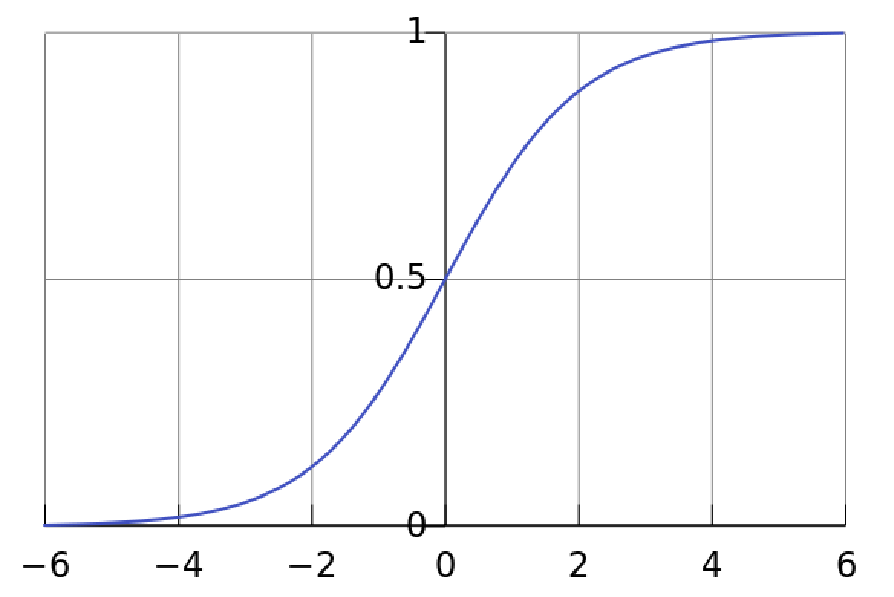
\includegraphics[scale=0.3]{figs/sigmoid}}
\pause
\item Non-linearity will be important in expressiveness multi-layer nets. Other non-linearities, e.g., $tanh(z)=(e^z-e^{-z}) / (e^z+e^{-z})$
\ei
\end{frame}


%%%%%%%%%%%%%
\begin{frame}
\frametitle{Gradient Descent for Logistic Regression }
\bi
\item Assume Squared-Error$^*$ $Loss(w) = \frac{1}{2} \sum_{m}  ( \sigma(w^T x^{(m)}) - y^{(m)} )^2$
\pause
%\item Gradient: $\nabla_w Loss = \sum_m {\color{red} ( \sigma(w^T x^{(m)}) - y^{(m)} )} {\color{blue} (\sigma(w^Tx^{(m)}) (1- \sigma(w^Tx^{(m)}) )} x^{(m)}$
\item Gradient: $\nabla_w Loss = \sum_m {\color{red} \left[ \sigma(w^T x^{(m)}) - y^{(m)} \right]} {\color{blue} \sigma'(w^Tx^{(m)})} x^{(m)}$
	\bi
	\pause
	\item Define input into non-linearity  ${\color{blue} in^{(m)} = w^Tx^{(m)}}$
	\item General form of gradient: $\sum_m{\color{red} Error^{(m)}} * {\color{blue} \sigma'(in^{(m)})} * x^{(m)}$
	\item Derivative of sigmoid $\sigma'(z) = \sigma(z) (1-\sigma(z))$
	\ei
\pause 
\item Gradient Descent Algorithm: 
	\be
	\item Initialize $w$ randomly
	\item Update until convergence: $w \leftarrow w - \gamma( \nabla_w Loss )$
	\ee
\item Stochastic gradient descent (SGD) algorithm:
	\be
	\item Initialize $w$ randomly
	\item Update until convergence: $w \leftarrow w - \gamma({\color{red} Error^{(m)}} * {\color{blue} \sigma'(in^{(m)})} * x^{(m)})$
	\ee
\ei
\vspace{-0.8cm}
\blfootnote{\hspace{-0.4cm}*An alternative is Cross-Entropy loss: $\sum_m~y^{(m)} \log(\sigma(w^Tx^{(m)}))+(1-y^{(m)}) \log(1-\sigma(w^Tx^{(m)}))$ }

\end{frame}

%%%%%%%%%%%%
\begin{frame}
\frametitle{Stochastic Gradient Descent (SGD)}
\bi
\item Gradient Descent Algorithm: 
	\be
	\item Initialize $w$ randomly
	\item Update until convergence: $w \leftarrow w - \gamma( \nabla_w Loss )$
	\ee
\item Stochastic gradient descent (SGD) algorithm:
	\be
	\item Initialize $w$ randomly
	\item Update until convergence: $w \leftarrow w - \gamma(\frac{1}{|B|}\sum_{m \in B}{\color{red} Error^{(m)}} * {\color{blue} \sigma'(in^{(m)})} * x^{(m)})$\\
          where minibatch $B$ ranges from e.g. 1-100 samples
	\ee
\pause
\item Learning rate $\gamma$:
  \bi
  \item For convergence, should decrease with each iteration $t$ through samples
  \item e.g. $\gamma_t = \frac{1}{\lambda * t} $ or $\gamma_t = \frac{\gamma_0}{1 + \gamma_0 * \lambda * t}$
  \ei
\ei

\end{frame}

%%%%%%%%%%%%%
\begin{frame}
\frametitle{SGD Pictorial View}
\bi
\item Loss objective contour plot: \begin{small}$\frac{1}{2} \sum_{m}  ( \sigma(w^T x^{(m)}) - y^{(m)} )^2 + ||w||$\end{small}
\bi
	\item Gradient descent goes in steepest descent direction
	\item SGD is noisy descent (but faster per iteration)
\ei
\ei
\centerline{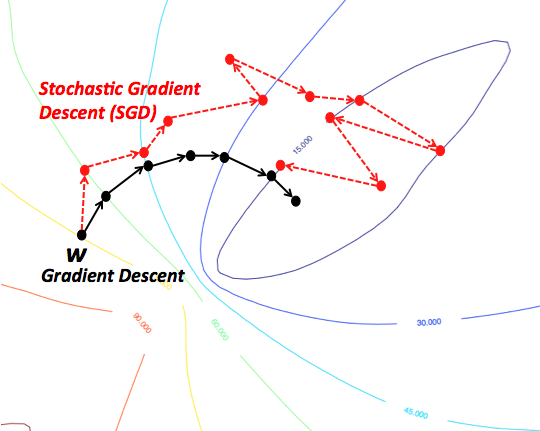
\includegraphics[scale=0.4]{figs/sgd_contour}}
\end{frame}


%%%%%%%%%%%%%
\begin{frame}
\frametitle{2-layer Neural Networks}
\begin{tikzpicture}[->,>=stealth',shorten >=1pt,auto,node distance=3cm,
  thick,main node/.style={circle,fill=blue!20,draw,font=\sffamily\Large\bfseries}]

  \node[main node] (1) at (1,0) {$x_1$};
  \node[main node] (2) at (3,0) {$x_2$};
  \node[main node] (3) at (5,0) {$x_3$};
  \node[main node] (4) at (7,0) {$x_4$};
  \node[main node] (h1) at (2,2) {$h_1$};
  \node[main node] (h2) at (4,2) {$h_2$};
  \node[main node] (h3) at (6,2) {$h_3$};
  \node[main node] (y) at (4,4) {$y$};

   \node(xi) at (0,0) {$x_i$};
   \node(wij) at (0,1) {${\color{red} w_{ij}}$};
   \node(hj) at (0,2) {$h_j$};
   \node(wj) at (0,3) {${\color{blue} w_{j}}$};

	

  \path[every node/.style={font=\sffamily\small}]
    (1) edge node [left] {${\color{red} w_{11}}$} (h1)
    (2) edge node {} (h1)
    (3) edge node {} (h1)
    (4) edge node {} (h1)
    (1) edge node [left] {${\color{red} w_{12}}$} (h2)
    (2) edge node {} (h2)
    (3) edge node {} (h2)
    (4) edge node {} (h2)
    (1) edge node {} (h3)
    (2) edge node {} (h3)
    (3) edge node {} (h3)
    (4) edge node {} (h3)
    (h1) edge node [left] {${\color{blue} w_1}$} (y)
    (h2) edge node [left] {${\color{blue} w_2}$} (y)
    (h3) edge node [left] {${\color{blue} w_3}$} (y)
    ;
\end{tikzpicture}

\vspace{4mm}
\begin{math}
f(x)=\sigma(\sum_j w_j \cdot h_j)
= \sigma(\sum_j {\color{blue} w_j} \cdot \sigma(\sum_i {\color{red} w_{ij}}  x_i))
\end{math}\\
\pause
\vspace{0.3cm}
Hidden units $h_j$'s can be viewed as new "features" from combining $x_i$'s
\blfootnote{\hspace{-0.5cm}Called Multilayer Perceptron (MLP), but more like multilayer logistic regression}
\end{frame}


%%%%%%%%%%%%%%%%
\begin{frame}
\frametitle{Expressive Power of Non-linearity}
\bi
\item A deeper architecture is more expressive than a shallow one given same number of nodes
\cite{bishop95book}
\bi
	\item 1-layer nets only model linear hyperplanes
	\item 2-layer nets can model any continuous function (given sufficient nodes)
	\item $>$3-layer nets can do so with fewer nodes
\ei
\ei
\centerline{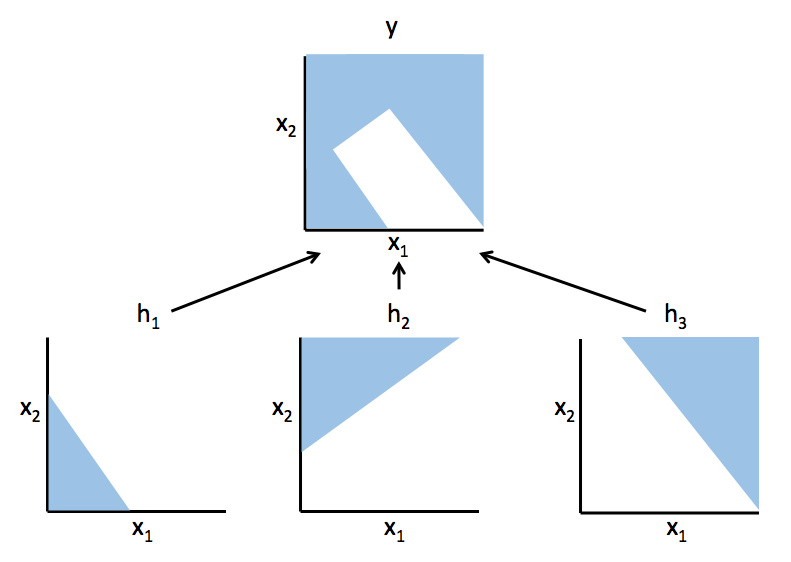
\includegraphics[scale=0.27]{figs/twolayer_nonlinearity}}
\end{frame}



%%%%%%%%%%%%%
\begin{frame}
\frametitle{Training Neural Nets: Back-propagation}
\begin{tikzpicture}[->,>=stealth',shorten >=1pt,auto,node distance=3cm,
  thick,main node/.style={circle,fill=blue!20,draw,font=\sffamily\Large\bfseries}]

  \node[main node] (1) at (1,0) {$x_1$};
  \node[main node] (2) at (3,0) {$x_2$};
  \node[main node] (3) at (5,0) {$x_3$};
  \node[main node] (4) at (7,0) {$x_4$};
  \node[main node] (h1) at (2,2) {$h_1$};
  \node[main node] (h2) at (4,2) {$h_2$};
  \node[main node] (h3) at (6,2) {$h_3$};
  \node[main node] (y) at (4,4) {$y$};

   \node(xi) at (0,0) {$x_i$};
   \node(wij) at (0,1) {$w_{ij}$};
   \node(hj) at (0,2) {$h_j$};
   \node(wj) at (0,3) {$w_{j}$};

	
  \draw[blue,ultra thick,-latex,->] (6.8,0.5) -- node[below right]{Predict $f(x^{(m)})$} (6.8,4);
  \draw[red,ultra thick,-latex,<-] (9.8,0.5) -- node[above left]{Adjust weights} (9.8,4);


  \path[every node/.style={font=\sffamily\small}]
    (1) edge node [left] {$w_{11}$} (h1)
    (2) edge node {} (h1)
    (3) edge node {} (h1)
    (4) edge node {} (h1)
    (1) edge node [left] {$w_{12}$} (h2)
    (2) edge node {} (h2)
    (3) edge node {} (h2)
    (4) edge node {} (h2)
    (1) edge node {} (h3)
    (2) edge node {} (h3)
    (3) edge node {} (h3)
    (4) edge node {} (h3)
    (h1) edge node [left] {$w_1$} (y)
    (h2) edge node [left] {$w_2$} (y)
    (h3) edge node [left] {$w_3$} (y)
    ;
\end{tikzpicture}

1. For each sample, compute $f(x^{(m)}) = \sigma(\sum_j w_j \cdot \sigma(\sum_i w_{ij}  x_i^{(m)}))$\\
2. If $f(x^{(m)})\ne y^{(m)}$, back-propagate error and adjust weights $\{w_{ij}, w_j\}$. 
\end{frame}

%%%%%%%%%%%%%
\begin{frame}
\frametitle{Derivatives of the weights}
Assume two outputs $(y_1, y_2)$ per input $x$,\\ and loss per sample:
$Loss = \sum_k \frac{1}{2} \left[ \sigma(in_k)   - y_k \right]^2 $

\begin{center}
\scalebox{0.7}{
\begin{tikzpicture}[->,>=stealth',shorten >=1pt,auto,node distance=3cm,
  thick,main node/.style={circle,fill=blue!20,draw,font=\sffamily\Large\bfseries}]

  \node[main node] (1) at (1,0) {$x_1$};
  \node[main node] (2) at (3,0) {$x_2$};
  \node[main node] (3) at (5,0) {$x_3$};
  \node[main node] (4) at (7,0) {$x_4$};
  \node[main node] (h1) at (2,2) {$h_1$};
  \node[main node] (h2) at (4,2) {$h_2$};
  \node[main node] (h3) at (6,2) {$h_3$};
  \node[main node] (y1) at (3,4) {$y_1$};
  \node[main node] (y2) at (5,4) {$y_2$};

 \node(xi) at (0,0) {$x_i$};
   \node(wij) at (0,1) {$w_{ij}$};
   \node(hj) at (0,2) {$h_j$};
   \node(wjk) at (0,3) {$w_{jk}$};
   \node(yk) at (0,4) {$y_{k}$};


  \path[every node/.style={font=\sffamily\small}]
    (1) edge node {} (h1)
    (2) edge node {} (h1)
    (3) edge node {} (h1)
    (4) edge node {} (h1)
    (1) edge node {} (h2)
    (2) edge node {} (h2)
    (3) edge node {} (h2)
    (4) edge node {} (h2)
    (1) edge node {} (h3)
    (2) edge node {} (h3)
    (3) edge node {} (h3)
    (4) edge node {} (h3)
    (h1) edge node {} (y1)
    (h2) edge node {}  (y1)
    (h3) edge node {} (y1)
    (h1) edge node {} (y2)
    (h2) edge node {}  (y2)
    (h3) edge node {} (y2)
    ;
\end{tikzpicture}
}
\end{center}

\pause
$ \frac{\partial Loss}{ \partial w_{jk}}
= {\color{red} \frac{\partial Loss}{ \partial in_k}} {\color{blue} \frac{ \partial in_k}{ \partial w_{jk}}}
= {\color{red} \delta_k} {\color{blue} \frac{\partial (\sum_j w_{jk} h_j)}{\partial w_{jk}} }
= {\color{red} \delta_k} {\color{blue} h_j}$

\pause
$ \frac{\partial Loss}{ \partial w_{ij}}
= {\color{red} \frac{\partial Loss}{ \partial in_j}} {\color{blue} \frac{ \partial in_j}{ \partial w_{ij}}}
= {\color{red} \delta_j} {\color{blue} \frac{\partial (\sum_j w_{ij} x_i)}{\partial w_{ij}} }
= {\color{red} \delta_j} {\color{blue} x_i}$

\pause
${\color{red} \delta_k = \frac{\partial}{\partial in_k} \left( \sum_k \frac{1}{2}  \left[ \sigma(in_k)   - y_k \right]^2\right)
= \left[ \sigma(in_k)-y_k \right] \sigma'(in_k) }$

\pause
${\color{red} \delta_j =  \sum_k  \frac{\partial Loss}{\partial in_k} \frac{\partial in_k}{\partial in_j} = \sum_k \delta_k
\cdot \frac{\partial}{\partial in_j}\left( \sum_j w_{jk} \sigma(in_j) \right) = \left[\sum_k \delta_k w_{jk}\right] \sigma'(in_j)}$


\end{frame}


%%%%%%%%%%%%%
\begin{frame}
\frametitle{Training Neural Nets: Back-propagation�}
All updates involve some {\color{red} scaled error from output} $*$ {\color{blue} input feature}:\\
\bi
\item $ \frac{\partial Loss}{ \partial w_{jk}} = {\color{red} \delta_k} {\color{blue} h_j}$
where ${\color{red} \delta_k = \left[ \sigma(in_k)-y_k \right] \sigma'(in_k) }$
\item $ \frac{\partial Loss}{ \partial w_{ij}} = {\color{red} \delta_j} {\color{blue} x_i}$
where ${\color{red} \delta_j = \left[\sum_k \delta_k w_{jk}\right] \sigma'(in_j)}$
\ei
First compute {\color{red} $\delta_k$} from final layer, then {\color{red} $\delta_j$} for previous layer and iterate.

\scalebox{1}{
\begin{tikzpicture}[->,>=stealth',shorten >=1pt,auto,node distance=3cm,
  thick,main node/.style={circle,fill=blue!20,draw,font=\sffamily\Large\bfseries}]

  \node[main node] (1) at (1,0) {$x_1$};
  \node[main node] (2) at (3,0) {$x_2$};
  \node[main node] (3) at (5,0) {$x_3$};
  \node[main node] (4) at (7,0) {$x_4$};
  \node[main node] (h1) at (2,2) {$h_1$};
  \node[main node] (h2) at (4,2) {$h_2$};
  \node[main node] (h3) at (6,2) {$h_3$};
  \node[main node] (y1) at (3,4) {$y_1$};
  \node[main node] (y2) at (5,4) {$y_2$};


   \node(xi) at (0,0) {$x_i$};
   \node(wij) at (0,1) {$w_{ij}$};
   \node(hj) at (0,2) {$h_j$};
   \node(wjk) at (0,3) {$w_{jk}$};
   \node(yk) at (0,4) {$y_{k}$};

   \node(deltah3) at (8.6,2.6) {${\color{red} \delta_{j=h_3} = [\delta_{k=y_1}w_{31} + \delta_{k=y_2}w_{32}]\sigma'(in_{h_3}) }$};
   \node(deltay1) at (4,4) {${\color{red} \delta_{k=y_1}}$};
   \node(deltay2) at (6,4) {${\color{red} \delta_{k=y_2}}$};

  \path[every node/.style={font=\sffamily\small}]
    (1) edge node {} (h1)
    (2) edge node {} (h1)
    (3) edge node {} (h1)
    (4) edge node {} (h1)
    (1) edge node {} (h2)
    (2) edge node {} (h2)
    (3) edge node {} (h2)
    (4) edge node {} (h2)
    (1) edge node {} (h3)
    (2) edge node {} (h3) 
    (3) edge node {} (h3)
    (4) edge node [right] {$ \frac{\partial Loss}{ \partial w_{ij}}$} (h3)
    (h1) edge node {} (y1)
    (h2) edge node {}  (y1)
    (h3) edge node [right] {${\color{red} w_{31}}$} (y1)
    (h1) edge node {} (y2)
    (h2) edge node {}  (y2)
    (h3) edge node [right] {${\color{red} w_{32}}$} (y2)
    ;
\end{tikzpicture}
}

\end{frame}

%% SUBSECTION%%%%%
\subsection[Computation Graph]{Computation Graphs and Deep Learning Toolkits}

%%%%%%%%%%%%%%%%
\begin{frame}
\frametitle{Current models are becoming more complex}
\vspace{0.5cm}
Do you want to take the derivative of this? \\
\vspace{0.5cm}
\centerline{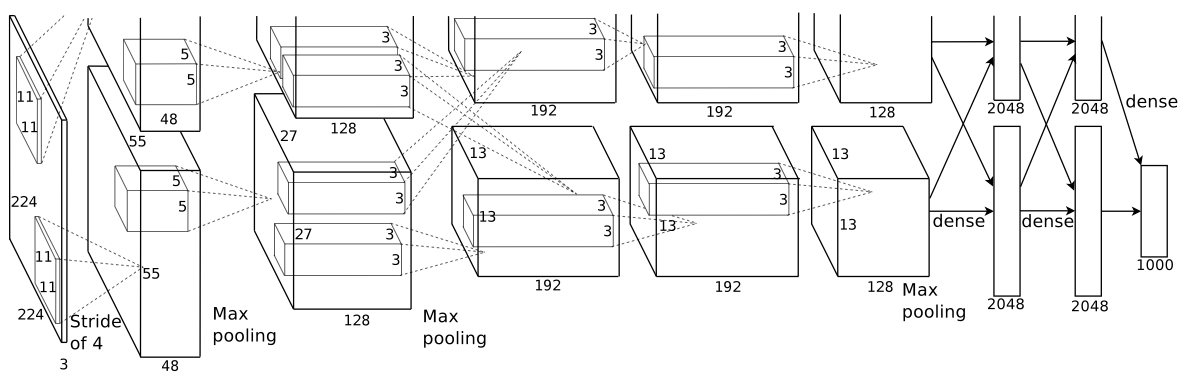
\includegraphics[scale=0.25]{figs/alexnet}}
\bi
\item AlexNet for image classification \cite{krizhevsky12imagenet}
\ei
\end{frame}

%%%%%%%%%%%%%%%%
\begin{frame}
\frametitle{Computation Graphs}
\bi
\item All computations can be viewed on a graph: 
\item e.g. 2-layer MLP: 
\begin{math}
y = softmax(W^{(2)} \cdot \sigma(W^{(1)}\cdot X+B^{(1)}) + B^{(2)}) 
\end{math}\\
\ei
\centerline{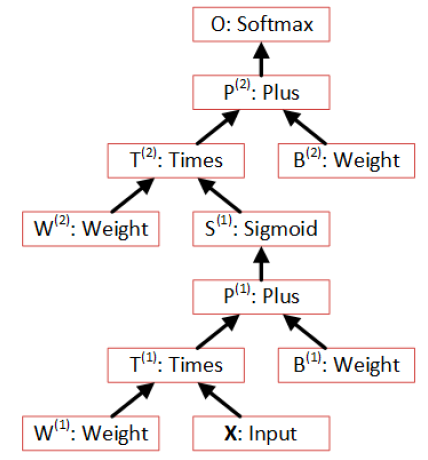
\includegraphics[scale=0.3]{figs/cntk1}}
\blfootnote{Figure from MSR CNTK tech report \cite{yu14cntk}\\\hspace{1cm} *$softmax(a_k)=\exp(a_k)/\sum_j\exp(a_j)$}
\end{frame}

%%%%%%%%%%%%%%%%
\begin{frame}
\frametitle{Computation Graphs}
\bi
\item All computations can be viewed on a graph: 
\item e.g. 2-layer MLP with {\color{red} shared weights}: 
\begin{math}
y = softmax(W^{(1)} \cdot \sigma(W^{(1)}\cdot X+B^{(1)}) + B^{(2)}) 
\end{math}\\
\ei
\centerline{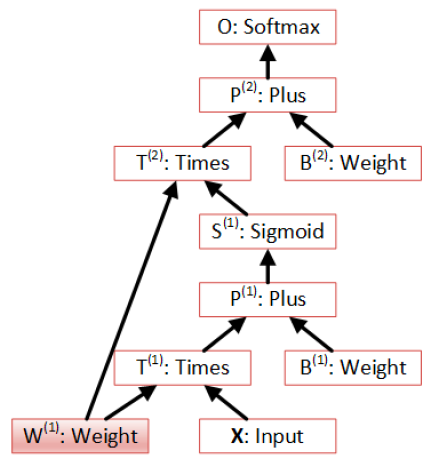
\includegraphics[scale=0.3]{figs/cntk2}}
\blfootnote{Figure from MSR CNTK tech report \cite{yu14cntk}\\\hspace{1cm} *$softmax(a_k)=\exp(a_k)/\sum_j\exp(a_j)$}
\end{frame}

%%%%%%%%%%%%%%%%
\begin{frame}
\frametitle{Computation Graphs}
\bi
\item All computations can be viewed on a graph: 
\item e.g. Computing the {\color{red} loss term} of the MLP
\ei
\centerline{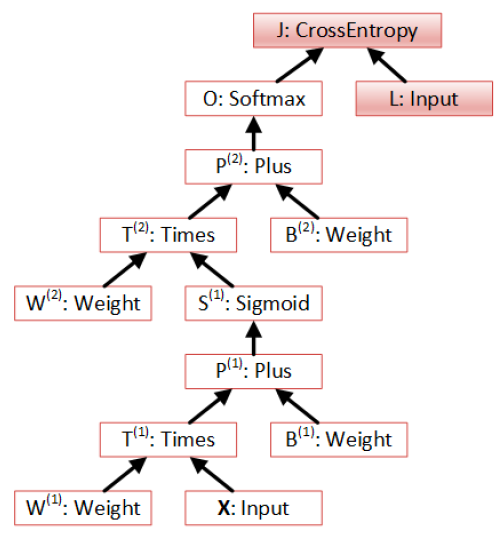
\includegraphics[scale=0.3]{figs/cntk3}}
\blfootnote{Figure from MSR CNTK tech report \cite{yu14cntk}\\\hspace{1cm} *$softmax(a_k)=\exp(a_k)/\sum_j\exp(a_j)$}
\end{frame}


%%%%%%%%%%%%%%%%
\begin{frame}
\frametitle{Toolkits enable rapid experimentation of various architectures}
Popular toolkits: Theano, Torch, pylearn2, Caffe, CNTK, CNN, Kaldi, etc.
\be
\item Compiles mathematical expression to graph
\item Implements basic operation for each node
\item Handles scheduling and batching of foward/backward computation
\item Also, GPU or fast math library support
\ee
\end{frame}


%% SUBSECTION%%%%%
\subsection[Why Deep is Hard]{Why Deep Architectures are Hard}

%%%%%%%%%%%%%%%%
\begin{frame}
\frametitle{Potential of Deep Architecture}
\begin{columns}
\begin{column}{0.5\textwidth}
\centerline{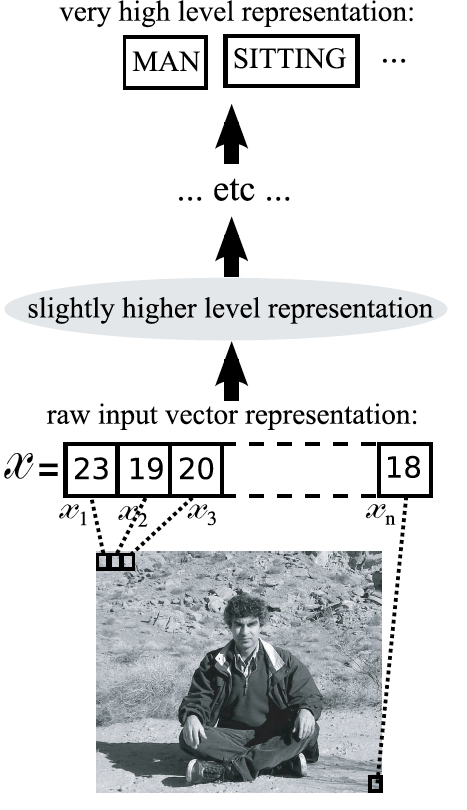
\includegraphics[scale=0.27]{figs/bengio_sitting}}
\textit{*Figure from \cite{bengio09book}}
\end{column}
\begin{column}{0.5\textwidth}
\begin{center}
\begin{tikzpicture}[-,>=stealth',shorten >=1pt,auto,node distance=3cm,
  thick,main node/.style={circle,fill=blue!20,draw,font=\sffamily\Large\bfseries}]

  \node[main node] (x1) at (0,0) {$x_1$};
  \node[main node] (x2) at (2,0) {$x_2$};
  \node[main node] (x3) at (4,0) {$x_3$};
  \node[main node] (h1) at (0,2) {$h_1$};
  \node[main node] (h2) at (2,2) {$h_2$};
  \node[main node] (h3) at (4,2) {$h_3$};
  \node[main node] (h'1) at (0,4) {$h'_1$};
  \node[main node] (h'2) at (2,4) {$h'_2$};
  \node[main node] (h'3) at (4,4) {$h'_3$};
  \node[main node] (y) at (2,6) {$y$};

  \path[every node/.style={font=\sffamily\small}]
    (x1) edge node {} (h1)
    (x1) edge node {} (h2)
    (x1) edge node {} (h3)
    (x2) edge node {} (h1)
    (x2) edge node {} (h2)
    (x2) edge node {} (h3)
    (x3) edge node {} (h1)
    (x3) edge node {} (h2)
    (x3) edge node {} (h3)
    (h1) edge node {} (h'1)
    (h1) edge node {} (h'2)
    (h1) edge node {} (h'3)
    (h2) edge node {} (h'1)
    (h2) edge node {} (h'2)
    (h2) edge node {} (h'3)
    (h3) edge node {} (h'1)
    (h3) edge node {} (h'2)
    (h3) edge node {} (h'3)
    (h'1) edge node {} (y)
    (h'2) edge node {} (y)
    (h'3) edge node {} (y) ;

\end{tikzpicture}
\end{center}
\end{column}
\end{columns}
\end{frame}


%%%%%%%%%%%%%%%%
\begin{frame}
\frametitle{Difficulties of Deep Architecture}
\begin{columns}
\begin{column}{0.5\textwidth}
\textbf{Vanishing gradient problem} in Backpropagation
\bi
\item $ \frac{\partial Loss}{ \partial w_{ij}} = {\color{red} \frac{\partial Loss}{ \partial in_j}} {\color{blue} \frac{ \partial in_j}{ \partial w_{ij}}}  = {\color{red} \delta_j}x_i$
\item ${\color{red} \delta_j =  \left[\sum_{j+1} \delta_{j+1} w_{j(j+1)}\right] \sigma'(in_j)}$
\item ${\color{red} \delta_j}$ may vanish after repeated multiplication
\item Also, exploding gradient problem!
\ei
\end{column}
\begin{column}{0.5\textwidth}
\begin{center}
\begin{tikzpicture}[-,>=stealth',shorten >=1pt,auto,node distance=3cm,
  thick,main node/.style={circle,fill=blue!20,draw,font=\sffamily\Large\bfseries}]

  \node[main node] (x1) at (0,0) {$x_1$};
  \node[main node] (x2) at (2,0) {$x_2$};
  \node[main node] (x3) at (4,0) {$x_3$};
  \node[main node] (h1) at (0,2) {$h_1$};
  \node[main node] (h2) at (2,2) {$h_2$};
  \node[main node] (h3) at (4,2) {$h_3$};
  \node[main node] (h'1) at (0,4) {$h'_1$};
  \node[main node] (h'2) at (2,4) {$h'_2$};
  \node[main node] (h'3) at (4,4) {$h'_3$};
  \node[main node] (y) at (2,6) {$y$};

   \node(wij) at (4.3,1) {${\color{red}w_{ij}}$};
   \node(wjj1) at (4.6,3) {${\color{red}w_{j(j+1)}}$};
   
  \path[every node/.style={font=\sffamily\small}]
    (x1) edge node {} (h1)
    (x1) edge node {} (h2)
    (x1) edge node {} (h3)
    (x2) edge node {} (h1)
    (x2) edge node {} (h2)
    (x2) edge node {} (h3)
    (x3) edge node {} (h1)
    (x3) edge node {} (h2)
    (x3) edge node {} (h3)
    (h1) edge node {} (h'1)
    (h1) edge node {} (h'2)
    (h1) edge node {} (h'3)
    (h2) edge node {} (h'1)
    (h2) edge node {} (h'2)
    (h2) edge node {} (h'3)
    (h3) edge node {} (h'1)
    (h3) edge node {} (h'2)
    (h3) edge node {} (h'3)
    (h'1) edge node {} (y)
    (h'2) edge node {} (y)
    (h'3) edge node {} (y) ;

\end{tikzpicture}
\end{center}
\end{column}
\end{columns}
\end{frame}



%%%%%%%%%%%%%%%%
\begin{frame}
\frametitle{Training Difficulties \cite{erhan09difficulty}}
\bi
\item MNIST digit classification task
\item Train neural net by Backpropagation (random initialization of $w_{ij}$) 
\ei 
\centerline{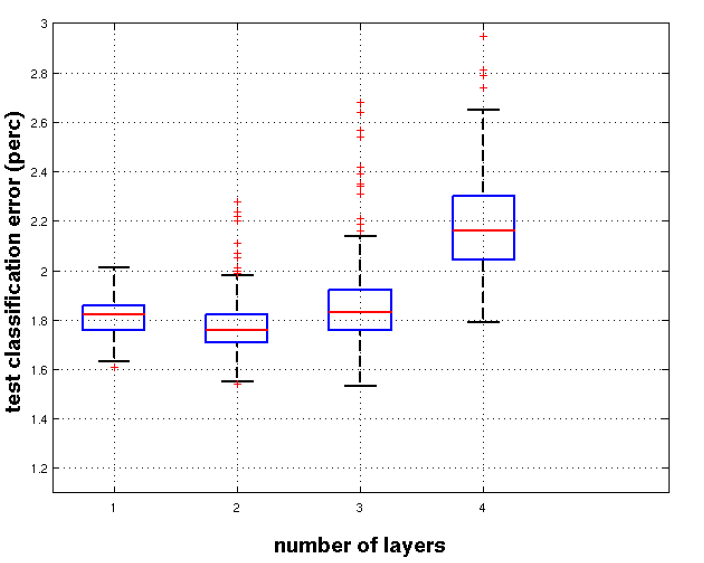
\includegraphics[scale=0.36]{figs/difficulty_backprop}}
\end{frame}



%% SUBSECTION%%%%%
\subsection[2006 Breakthrough]{The Breakthrough in 2006}

%%%%%%%%%%%%%%%%
\begin{frame}
\frametitle{Layer-wise Pre-training \cite{hinton06dbn}}
First, train one layer at a time, optimizing data-likelihood objective $P(x)$
\begin{center}
\begin{tikzpicture}[-,>=stealth',shorten >=1pt,auto,node distance=3cm,
  thick,main node/.style={circle,fill=blue!20,draw,font=\sffamily\Large\bfseries}]

  \node[main node] (x1) at (0,0) {$x_1$};
  \node[main node] (x2) at (2,0) {$x_2$};
  \node[main node] (x3) at (4,0) {$x_3$};
  \node[main node] (h1) at (0,2) {$h_1$};
  \node[main node] (h2) at (2,2) {$h_2$};
  \node[main node] (h3) at (4,2) {$h_3$};
  \node[main node] (h'1) at (0,4) {$h'_1$};
  \node[main node] (h'2) at (2,4) {$h'_2$};
  \node[main node] (h'3) at (4,4) {$h'_3$};
  \node[main node] (y) at (2,6) {$y$};

  \draw[blue,ultra thick,-latex,<->] (5,0) -- node[right]{Train Layer1} (5,2);


  \path[every node/.style={font=\sffamily\small}]
    (x1) edge node {} (h1)
    (x1) edge node {} (h2)
    (x1) edge node {} (h3)
    (x2) edge node {} (h1)
    (x2) edge node {} (h2)
    (x2) edge node {} (h3)
    (x3) edge node {} (h1)
    (x3) edge node {} (h2)
    (x3) edge node {} (h3)
    (h1) edge node {} (h'1)
    (h1) edge node {} (h'2)
    (h1) edge node {} (h'3)
    (h2) edge node {} (h'1)
    (h2) edge node {} (h'2)
    (h2) edge node {} (h'3)
    (h3) edge node {} (h'1)
    (h3) edge node {} (h'2)
    (h3) edge node {} (h'3)
    (h'1) edge node {} (y)
    (h'2) edge node {} (y)
    (h'3) edge node {} (y) ;

\end{tikzpicture}
\end{center}
\end{frame}



%%%%%%%%%%%%%%%%
\begin{frame}
\frametitle{Layer-wise Pre-training \cite{hinton06dbn}}
First, train one layer at a time, optimizing data-likelihood objective $P(x)$
\begin{center}
\begin{tikzpicture}[-,>=stealth',shorten >=1pt,auto,node distance=3cm,
  thick,main node/.style={circle,fill=blue!20,draw,font=\sffamily\Large\bfseries}]

  \node[main node] (x1) at (0,0) {$x_1$};
  \node[main node] (x2) at (2,0) {$x_2$};
  \node[main node] (x3) at (4,0) {$x_3$};
  \node[main node] (h1) at (0,2) {$h_1$};
  \node[main node] (h2) at (2,2) {$h_2$};
  \node[main node] (h3) at (4,2) {$h_3$};
  \node[main node] (h'1) at (0,4) {$h'_1$};
  \node[main node] (h'2) at (2,4) {$h'_2$};
  \node[main node] (h'3) at (4,4) {$h'_3$};
  \node[main node] (y) at (2,6) {$y$};

  \draw[blue,ultra thick,-latex,<->] (5,2) -- node[right]{Train Layer2} (5,4);
  \draw[blue,ultra thick,-latex,<->] (5,0) -- node[right]{Keep Layer1 fixed} (5,2);

  \path[every node/.style={font=\sffamily\small}]
    (x1) edge node {} (h1)
    (x1) edge node {} (h2)
    (x1) edge node {} (h3)
    (x2) edge node {} (h1)
    (x2) edge node {} (h2)
    (x2) edge node {} (h3)
    (x3) edge node {} (h1)
    (x3) edge node {} (h2)
    (x3) edge node {} (h3)
    (h1) edge node {} (h'1)
    (h1) edge node {} (h'2)
    (h1) edge node {} (h'3)
    (h2) edge node {} (h'1)
    (h2) edge node {} (h'2)
    (h2) edge node {} (h'3)
    (h3) edge node {} (h'1)
    (h3) edge node {} (h'2)
    (h3) edge node {} (h'3)
    (h'1) edge node {} (y)
    (h'2) edge node {} (y)
    (h'3) edge node {} (y) ;

\end{tikzpicture}
\end{center}
\end{frame}

%%%%%%%%%%%%%%%%
\begin{frame}
\frametitle{Layer-wise Pre-training \cite{hinton06dbn}}
Finally, fine-tune labeled objective $P(y|x)$ by Backpropagation
\begin{center}
\begin{tikzpicture}[-,>=stealth',shorten >=1pt,auto,node distance=3cm,
  thick,main node/.style={circle,fill=blue!20,draw,font=\sffamily\Large\bfseries}]

  \node[main node] (x1) at (0,0) {$x_1$};
  \node[main node] (x2) at (2,0) {$x_2$};
  \node[main node] (x3) at (4,0) {$x_3$};
  \node[main node] (h1) at (0,2) {$h_1$};
  \node[main node] (h2) at (2,2) {$h_2$};
  \node[main node] (h3) at (4,2) {$h_3$};
  \node[main node] (h'1) at (0,4) {$h'_1$};
  \node[main node] (h'2) at (2,4) {$h'_2$};
  \node[main node] (h'3) at (4,4) {$h'_3$};
  \node[main node] (y) at (2,6) {$y$};

  \draw[red,ultra thick,-latex,->] (5,0) -- node[below right]{Predict f(x)} (5,6);
  \draw[red,ultra thick,-latex,->] (8,6) -- node[above left]{Adjust weights} (8,0);

  \path[every node/.style={font=\sffamily\small}]
    (x1) edge node {} (h1)
    (x1) edge node {} (h2)
    (x1) edge node {} (h3)
    (x2) edge node {} (h1)
    (x2) edge node {} (h2)
    (x2) edge node {} (h3)
    (x3) edge node {} (h1)
    (x3) edge node {} (h2)
    (x3) edge node {} (h3)
    (h1) edge node {} (h'1)
    (h1) edge node {} (h'2)
    (h1) edge node {} (h'3)
    (h2) edge node {} (h'1)
    (h2) edge node {} (h'2)
    (h2) edge node {} (h'3)
    (h3) edge node {} (h'1)
    (h3) edge node {} (h'2)
    (h3) edge node {} (h'3)
    (h'1) edge node {} (y)
    (h'2) edge node {} (y)
    (h'3) edge node {} (y) ;

\end{tikzpicture}
\end{center}
\end{frame}

%%%%%%%%%%%%%%%%
\begin{frame}
\frametitle{Layer-wise Pre-training \cite{hinton06dbn}}
\textbf{Key Idea:\\
Focus on modeling the input $P(X)$ better with each successive layer.\\
Worry about optimizing the task $P(Y|X)$ later.}
\begin{quote}\color{blue}{"If you want to do computer vision, first learn computer graphics." -- Geoff Hinton} \end{quote}

\begin{columns}
\begin{column}{0.7\textwidth}
\begin{center}
\scalebox{0.7}{
\begin{tikzpicture}[-,>=stealth',shorten >=1pt,auto,node distance=3cm,
  thick,main node/.style={circle,fill=blue!20,draw,font=\sffamily\Large\bfseries}]

  \node[main node] (x1) at (0,0) {$x_1$};
  \node[main node] (x2) at (2,0) {$x_2$};
  \node[main node] (x3) at (4,0) {$x_3$};
  \node[main node] (h1) at (0,2) {$h_1$};
  \node[main node] (h2) at (2,2) {$h_2$};
  \node[main node] (h3) at (4,2) {$h_3$};
  \node[main node] (h'1) at (0,4) {$h'_1$};
  \node[main node] (h'2) at (2,4) {$h'_2$};
  \node[main node] (h'3) at (4,4) {$h'_3$};
  \node[main node] (y) at (2,6) {$y$};

  \draw[blue,ultra thick,-latex,<->] (5,2) -- node[right]{Train Layer2} (5,4);
  \draw[blue,ultra thick,-latex,<->] (5,0) -- node[right]{Train Layer1} (5,2);

  \path[every node/.style={font=\sffamily\small}]
    (x1) edge node {} (h1)
    (x1) edge node {} (h2)
    (x1) edge node {} (h3)
    (x2) edge node {} (h1)
    (x2) edge node {} (h2)
    (x2) edge node {} (h3)
    (x3) edge node {} (h1)
    (x3) edge node {} (h2)
    (x3) edge node {} (h3)
    (h1) edge node {} (h'1)
    (h1) edge node {} (h'2)
    (h1) edge node {} (h'3)
    (h2) edge node {} (h'1)
    (h2) edge node {} (h'2)
    (h2) edge node {} (h'3)
    (h3) edge node {} (h'1)
    (h3) edge node {} (h'2)
    (h3) edge node {} (h'3)
    (h'1) edge node {} (y)
    (h'2) edge node {} (y)
    (h'3) edge node {} (y) ;

\end{tikzpicture}}
\end{center}
\end{column}
\begin{column}{0.3\textwidth}
\pause
\textit{Extra advantage:\\Can exploit large amounts of unlabeled data!}
\end{column}
\end{columns}
\end{frame}


\begin{frame}
\frametitle{Why does Pre-Training work?}
\begin{columns}
\begin{column}{0.4\textwidth}
\begin{center}
\scalebox{0.7}{
\begin{tikzpicture}[-,>=stealth',shorten >=1pt,auto,node distance=3cm,
  thick,main node/.style={circle,fill=blue!20,draw,font=\sffamily\Large\bfseries}]

  \node[main node] (x1) at (0,0) {$x_1$};
  \node[main node] (x2) at (2,0) {$x_2$};
  \node[main node] (x3) at (4,0) {$x_3$};
  \node[main node] (h1) at (0,2) {$h_1$};
  \node[main node] (h2) at (2,2) {$h_2$};
  \node[main node] (h3) at (4,2) {$h_3$};
  \node[main node] (h'1) at (0,4) {$h'_1$};
  \node[main node] (h'2) at (2,4) {$h'_2$};
  \node[main node] (h'3) at (4,4) {$h'_3$};
  \node[main node] (y) at (2,6) {$y$};

  \path[every node/.style={font=\sffamily\small}]
    (x1) edge node {} (h1)
    (x1) edge node {} (h2)
    (x1) edge node {} (h3)
    (x2) edge node {} (h1)
    (x2) edge node {} (h2)
    (x2) edge node {} (h3)
    (x3) edge node {} (h1)
    (x3) edge node {} (h2)
    (x3) edge node {} (h3)
    (h1) edge node {} (h'1)
    (h1) edge node {} (h'2)
    (h1) edge node {} (h'3)
    (h2) edge node {} (h'1)
    (h2) edge node {} (h'2)
    (h2) edge node {} (h'3)
    (h3) edge node {} (h'1)
    (h3) edge node {} (h'2)
    (h3) edge node {} (h'3)
    (h'1) edge node {} (y)
    (h'2) edge node {} (y)
    (h'3) edge node {} (y) ;

\end{tikzpicture}
}
\end{center}

\end{column}
\begin{column}{0.6\textwidth}
\bi
\item \cite{erhan10pretrain} - A deep net can fit the training data in many ways (non-convex):
	\be
	\item By optimizing upper-layers 
	\item By optimizing lower-layers 
	\ee
\pause
\item Top-down vs. Bottom-up information
	\be
	\item Even if lower-layers are random weights, upper-layer may still fit well. But may not generalize to new data
	\item Pre-training with objective on $P(x)$ learns more generalizable features
	\ee
\pause
\item Pre-training maybe put weights at a better local optimum
\ei
\end{column}
\end{columns}
\end{frame}



%%%%%%%%%%%%%%%%
\begin{frame}
\frametitle{Is Pre-Training really necessary?}
\pause
Answer in 2006: Yes!

\pause
Answer now: No!
\bi
\item On large data, back-prop seems to work. 
\item Clever architectures avoid vanishing/exploding gradient
\item While pre-training may not be needed for training deep architectures, they may help anyway (e.g. word embeddings for neural net parsers \cite{chen14depparse}).
\ei
\pause
\vspace{1cm}
{\color{red} Lesson: What we believe true today may not be true tomorrow. Don't follow dogma.} 
\end{frame}

%%%%%%%%%%%%%
\begin{frame}
\frametitle{Section Summary}
\bi
\item Neural Networks (1-layer, 2-layer) 
\item Computation Graphs and Deep Learning Toolkits
\item Why Deep Architectures are Hard
\item The Breakthrough in 2006
\ei
\end{frame}
